\newpage
\subsubsection{Supermario (by Philipp Haller)}

This part discusses the model used to solve a level of the Supermario game which was presented in section XX. 

The first entity modelled was the supermario wrapper which is closely related to the outputs and inputs of the simulator. Therefore it receives all necessary values as input with the aim to forward them to the actual controller and its corresponding sub-components. After computation the results of the controller are handed back into the wrapper, which forwards the data to the simulator. Figure XX shows the graphical representation, while listing XX shows the actual EMA implementation.
\begin{figure}
	\centering
	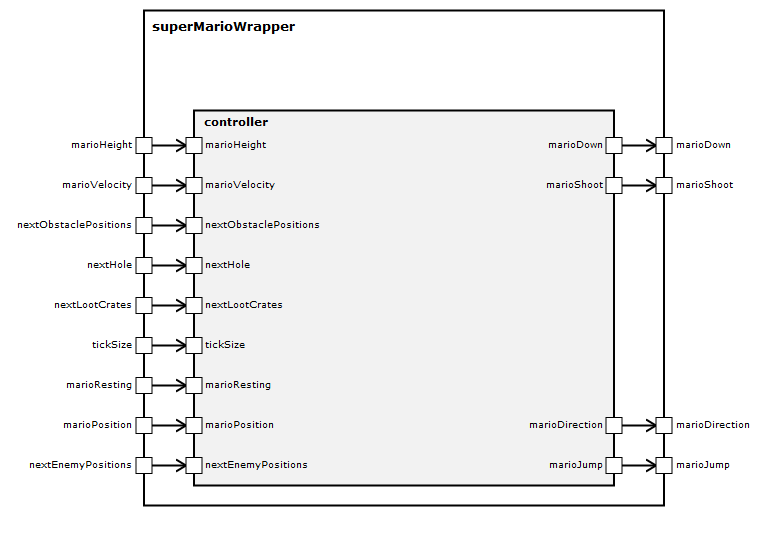
\includegraphics[scale=0.5]{pictures/haller_supermariowrapper.PNG}
	\caption{Visualisation of the Supermario wrapper model}
	\label{fig:marioWrapper}
\end{figure}

\begin{lstlisting}[label=lst:marioWrapperInterface, caption=Interface of the Supermario Wrapper, morekeywords={ports, port, connect, in, out, instance, ->},
frame=single]
    ports   
        in Z^{1,2} marioPosition,
        in Z^{1,2} marioVelocity,
        in Z marioHeight,
        in Z^{5,2} nextEnemyPositions,
        in Z^{5,2} nextObstaclePositions,
        in Z nextHole,
        in Z^{5,2} nextLootCrates,
        in Q tickSize,
        in Z marioResting,
        out Z(-1 : 1 : 1) marioDirection,
        out Z marioJump,
        out Z marioDown,
        out Z marioShoot;
\end{lstlisting}

\begin{lstlisting}[label=lst:marioWrapper, caption=Connectors of the Supermario Wrapper, morekeywords={ports, port, connect, in, out, instance, ->},
frame=single]
    instance Controller controller;
    
    connect marioPosition -> controller.marioPosition;
    connect marioVelocity -> controller.marioVelocity;
    connect marioHeight -> controller.marioHeight;
    connect nextEnemyPositions -> controller.nextEnemyPositions;
    connect nextObstaclePositions -> controller.nextObstaclePositions;
    connect nextHole -> controller.nextHole;
    connect nextLootCrates -> controller.nextLootCrates;
    connect tickSize -> controller.tickSize;
    connect marioResting -> controller.marioResting;
    
    connect controller.marioJump -> marioJump;
    connect controller.marioDirection -> marioDirection;
    connect controller.marioDown -> marioDown;
    connect controller.marioShoot -> marioShoot;
\end{lstlisting}

The inputs range from ... ... ... and the outputs .. .. are used to control the player's avatar.
<<detail nr. 1 .. n >>

DONT FORGET TO GIVE DEFINITIONS!
The controller consists of 5 parts. Two are sub-controllers tasked to cope with the evaluation of enemies and obstacles respectively.

During modelling of Supermario a distinction between models named with "controller" and "strategy was made.
In scope of the Supermario model the name "controller" was used to describe a model which 

The term "strategy" was used for a model which uses only atomic models and returns a action related advice 

"Watcher"

"Selector"

"Strategy"

"Controller"

"Decider??"

\begin{figure}
	\centering
	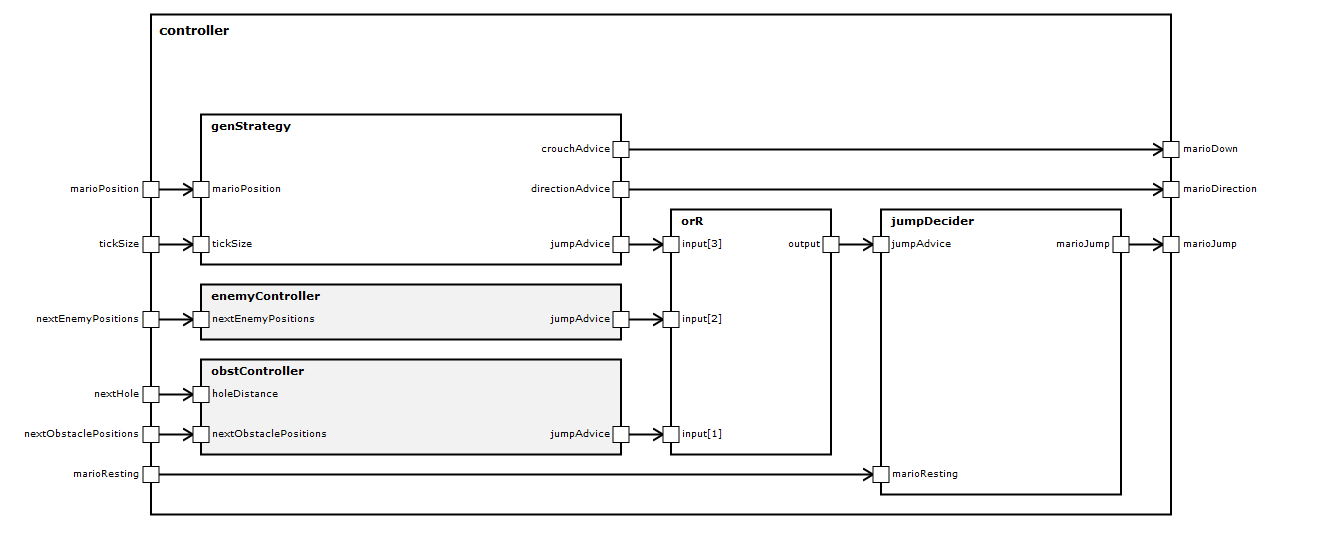
\includegraphics[scale=0.5]{pictures/haller_controller.PNG}
	\caption{Visualisation of the Supermario controller model}
	\label{fig:marioController}
\end{figure}

\begin{figure}
	\centering
	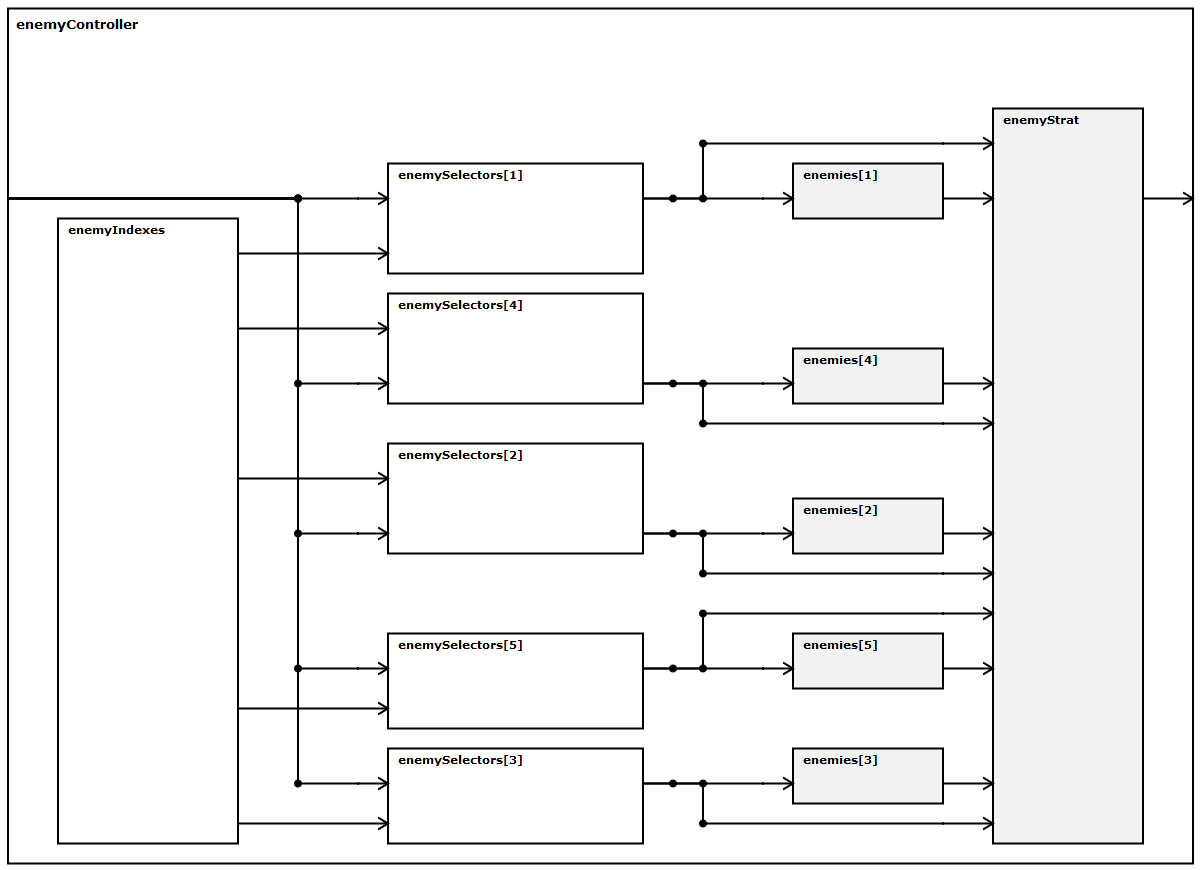
\includegraphics[scale=0.4]{pictures/haller_enemycontroller.PNG}
	\caption{Visualisation of the Supermario enemy controller model}
	\label{fig:marioEnemyController}
\end{figure}

\begin{figure}
	\centering
	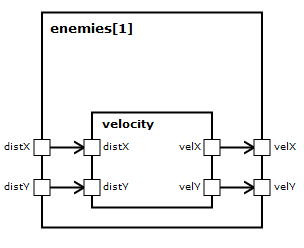
\includegraphics[scale=0.5]{pictures/haller_enemy.PNG}
	\caption{Visualisation of the Supermario enemy model}
	\label{fig:marioEnemy}
\end{figure}

\begin{figure}
	\centering
	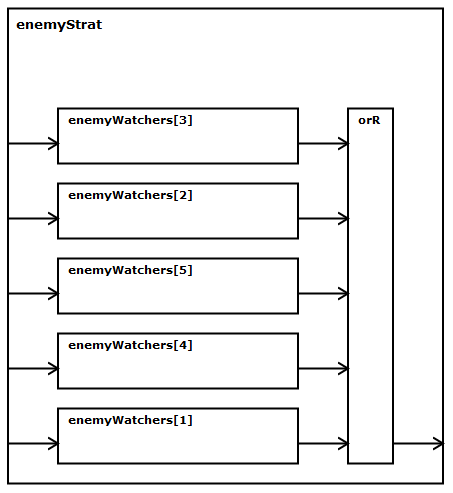
\includegraphics[scale=0.4]{pictures/haller_enemystrategy.PNG}
	\caption{Visualisation of the Supermario enemy strategy model}
	\label{fig:marioEnemyStrategy}
\end{figure}


\emph{Execution}

The presented models are executed in